\documentclass[aps,prb,showpacs,amsmath,amssymb,superscriptaddress]{revtex4-2}
%\documentclass[aps,prb,showpacs,twocolumn,amsmath,amssymb,superscriptaddress]{revtex4-2}
\bibliographystyle{apsrev4-2}

\usepackage{tabularx}
\usepackage{bm}
%\usepackage[demo]{graphicx}
\usepackage{graphicx}
\usepackage{tikz}

\usepackage{hyperref}
\hypersetup{colorlinks=true,urlcolor= blue,citecolor=blue,linkcolor= blue,bookmarks=true,bookmarksopen=false}

\usepackage{color}

\usepackage{amsmath,mathtools}
\usepackage{multirow}
\usepackage{dcolumn}
\usepackage{amssymb,amscd,xypic,bm,wasysym}
\usepackage{float}
\usepackage{cleveref}
\usepackage[caption=false,position=top,captionskip=0pt,farskip=0pt]{subfig}
\captionsetup[subfigure]{justification=raggedright,singlelinecheck=false}


\newcommand{\Red}[1]{\textcolor{red}{#1}}
%\newcommand{\vb}[1]{\boldsymbol{#1}}
\usepackage{soul}

% reset vec and hat style to a bold type
\let\oldhat\hat
\renewcommand{\hat}[1]{\oldhat{\mathbf{#1}}}
\renewcommand{\vec}[1]{\mathbf{#1}}
% stretches the vertical spacing of arrays/matrices
\renewcommand{\arraystretch}{1.5}
\setlength{\jot}{10pt}

\newcommand{\ham}{\mathcal{H}}
\newcommand{\cc}{c^{\dagger}}
\newcommand{\de}{\Delta}

\begin{abstract}
  \Red{PLACEHOLDER**APS MM 2022 Abstract}
  We study the possibility of obtaining robust Majorana modes at the corners of triangular islands of different superconductor models, with the goal of finding alternative structures that can serve as building blocks of topological quantum computation.
  By considering both spinless p-wave and ferromagnetic Rashba s-wave superconductor models on an equilateral triangle subject to inhomogeneous supercurrents, we found that Majorana corner modes can generally appear if the system being considered can be made equivalent to a triangular chain model, which can be understood by calculating the bulk Z2 topological invariant.
  We also discussed the robustness of the corner modes in possible experimental realizations of the triangular islands.
\end{abstract}

\begin{document}

\title{Superconducting triangular islands as a platform for manipulating Majorana fermions}

\author{Aidan Winblad}
\affiliation{Department of Physics, Colorado State University, Fort Collins, CO 80523, USA}

\author{Hua Chen}
\affiliation{Department of Physics, Colorado State University, Fort Collins, CO 80523, USA}
\affiliation{School of Advanced Materials Discovery, Colorado State University, Fort Collins, CO 80523, USA}

\maketitle



\section{Introduction}
\Red{1) Designs based on the kitaev chains and experimental evidence.}

\Red{2) Geometries different from chain, quasi-1D, 2D options}

\Red{3) Supercurrent and TSC}

random words

\Red{OUTLINE: (Sec I is \dots, Sec II is \dots)}
\section{Topological phase diagram of a finite width ribbon}

It has been previously shown that a constant vector potential can induce a topological phase transition for a spinless $p$-wave superconducting chain \cite{takasanSupercurrentinducedTopologicalPhase2022}, and other types of superconductors.
It appears Majorana fermions can behosted at the end points of a chain with finite width as with a Josephson-junction as seen in [REF], provided the width is much smaller than the Majorana fermion decay length.
Expanding on these ideas we would like to induce a topological phase transition for an infinite triangular lattice ribbon.
This will help create an argument using bulk-edge correspondence to inform how Majorana fermions will form at the interfaces of triangular island edges.

Let us start with the Hamiltonian of a spinless or spin-polarized $p$-wave superconductor of a triangular lattice
\begin{equation}
  \ham = \sum_{\langle j, l \rangle} (-t\cc_{l} c_j + \de e^{i\theta_{l,j}} \cc_{l}\cc_j + h.c.) - \sum_{j} \mu \cc_j c_j,
\end{equation}
where $t$ is the hopping amplitude, $\de$ is the superconducting order parameter, $\mu$ is the chemical potential, $\theta_{l,j}$ is the angle between sites $l$ and $j$.
Next, we will apply Peierls substitution to our creation(annihilation) operators
\begin{align}
  \cc_{l} c_j &\rightarrow \cc_{l} c_j \exp \left(-\dfrac{i e}{\hbar} \int_{r_j}^{r_{l}} \vec{A} \cdot d\vec{l} \right) \\ \nonumber
  &\rightarrow \cc_{l} c_j e^{i \phi_{l,j}}.
\end{align}
Here the electron charge, $e$, and Planck's constant, $\hbar$, will be treated as natural numbers.
The vector potential will be constant throughout the ribbon allowing for translational symmetry along the $x$-axis.
One finds that $t$ is the only term that picks up a phase, thus our modified Hamiltonian looks like
\begin{equation} \label{eq: Peierls Hamiltonian}
  \ham = \sum_{\langle j,l \rangle} (-t e^{i\phi_{l,j}} \cc_{l} c_j + \de e^{i\theta_{l,j}} \cc_{l}\cc_j + h.c.) - \sum_j \mu \cc_j c_j.
\end{equation}

Since we are interested how an infinite ribbon behaves in a vector field we will fourier transform along the $x$-axis only.
We pick the following transform to be
\begin{equation}
  \cc_{m,n} = \dfrac{1}{\sqrt{N}} \sum_{k} \cc_{k,n} e^{i \vec{k}\cdot\vec{r}_m}
\end{equation}
where $\vec{k}=k\hat{x}$ and $\vec{r}_m = ma\hat{x}$, and for convenience $a$ will be treated as a natural number, too.
This leads to the following block Hamiltonian
\begin{equation}
  \ham(k) = \dfrac{1}{2} \sum_k \Psi_k^\dagger \left(
    \begin{matrix}
      \epsilon(k) & \delta(k) \\
      \delta^\dagger(k) & -\epsilon(-k)
    \end{matrix} \right)
    \Psi_k.
\end{equation}
The $\epsilon(k)$ block is a tridiagonal with $\epsilon_0(k) = -2t\cos(k+\phi_1) - \mu$ along the diagonal, the upper diagonal is  $\epsilon_1(k) = -t(e^{-i\phi_2}+e^{i(k-\phi_3)})$, and $\epsilon_1^*(k)$ along the lower diagonal.
The $\delta(k)$ block is a tridiagonal with $\delta_0(k) = 2i\de \sin k $ along the diagonal, the upper diagonal is  $\delta_1(k) = -\de (e^{i\theta_2}+e^{i(k+\theta_3)})$, and $-\delta_1(-k)$ along the lower diagonal.
The size of each block is the number of rows along the $y$-axis in the infinite ribbon.

To calculate the Majorana number we need to rewrite our Hamiltonian to be in skew-symmetric form.
One such way is to write it in the Majorana fermion basis, the transformation matrix is of the form
\begin{equation}
  u = \dfrac{1}{\sqrt{2}} \left(
  \begin{matrix}
    1 & 1 \\
    -i & i
  \end{matrix} \right)
\end{equation}

To account for the finite number of rows in our ribbon we simply include a tensor product with an identity matrix of the same size, $U = u \otimes I_n$.
We can now arrive at the skew-symmetric matrix with the following equation
\begin{equation}
  A_{ch} = -i U \ham_{ch} U^{\dagger}.
\end{equation}
The Majorana number, $\mathcal{M}$, of a 1D chain is defined as
\begin{equation}
  \mathcal{M} = \text{sgn}[\text{Pf}(A_{ch})],
\end{equation}
where $\text{Pf}$ stands for the Pfaffian of a skew-symmetric matrix.
We make the claim this satisfies a finite width ribbon as well.
When $\mathcal{M} = -1$, the ribbon is in a non-trivial topology and we would expect Majorana zero modes at its edges.
As we sweep through a range of $A$ for our vector potential we expect to see a gap closing, $\mathcal{M} = 1$, and our system take on a trivial topology, thus no Majorana zero modes would exist on the edge of a finite ribbon.

To illustrate the importance of bulk-edge correspondence in forming Majorana fermions we will now look at the edges of a hollow triangular island.
We want to show the top edges can be in a trivial phase while the bottom remains in a non-trivial phase.
In previous papers a constant vector potential was used along the chain's axis.
If instead we use a constant vector potential step function centered on a chain with a 60 degree bend, equating it to a equilateral triangle, we can have an equivalent system to the chain model.
One also finds that the vector potential has symmetry about the ribbon's axis, i.e. $\vec{A}$ pointing in the positive or negative y-axis yields the same result.
Taking a hollow triangular island centered about the y-axis with the following vector potential
\begin{equation}
  \vec{A} = \begin{cases}
            A \hat{y} \quad &x > 0 \\
            -A \hat{y} \quad &x < 0 \\
            \end{cases}
\end{equation}
we can examine each edge individually.
Looking at figure \ref{fig: triangular-island-vector-potential-divided} we can quickly determine each edge's vector potential with respect to its main axis.

\begin{figure}[]
  \begin{tikzpicture}
    \node[inner sep=0pt] (figure) at (0,0){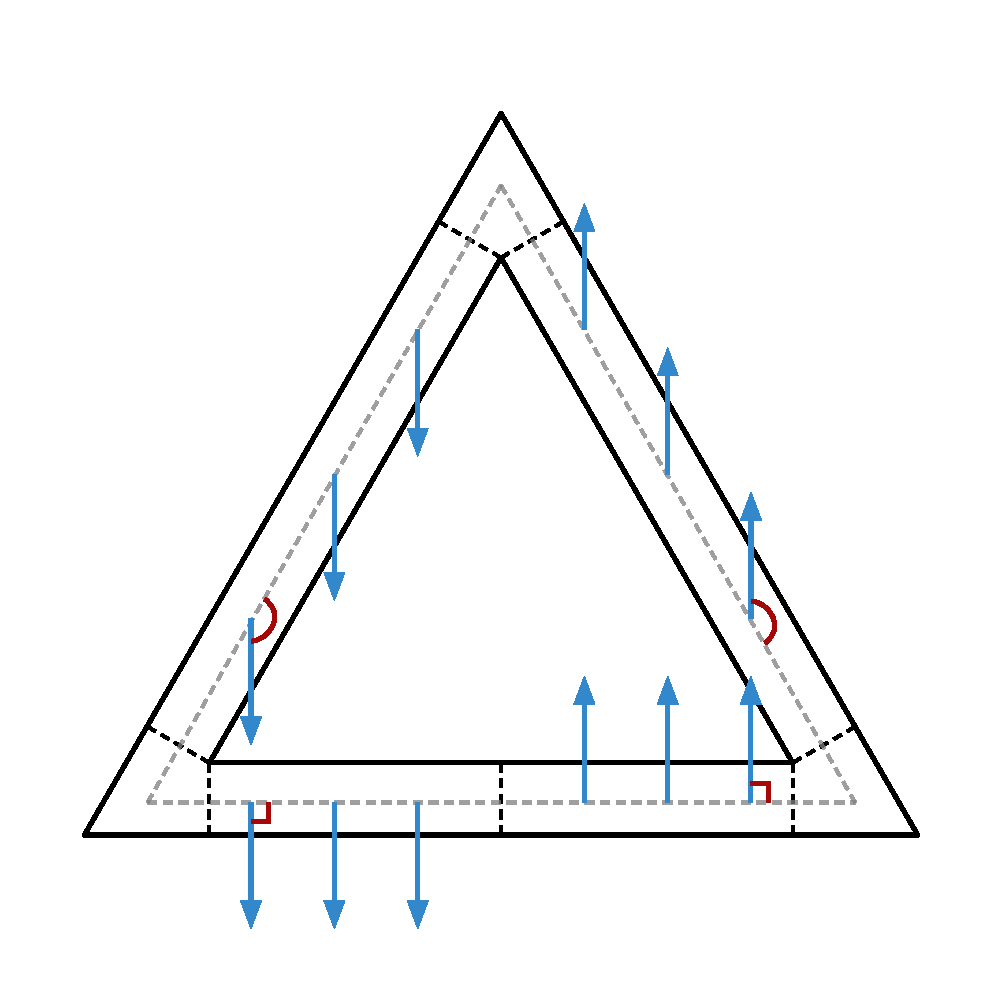
\includegraphics[width=0.5\textwidth]{./figures/triangular-island-vector-potential-divided.pdf}};
    \node[inner sep=0pt] (angle 1) at (-1.1,-1.1) {\small $\eta = -\dfrac{5\pi}{6}$};
    \node[inner sep=0pt] (angle 2) at (3.3,-1.0) {\small $\eta = \dfrac{5\pi}{6}$};
    \node[inner sep=0pt] (R1) at (-2.3,0.5) {\small I};
    \node[inner sep=0pt] (R2) at (2.3,0.5) {\small II};
    \node[inner sep=0pt] (R3) at (1.3,-3.3) {\small III};
    \node[inner sep=0pt] (R3) at (-1.3,-2.1) {\small IV};
  \end{tikzpicture}
  \label{fig: triangular-island-vector-potential-divided}
  \caption{Triangular island with constant step function vector potential. The edges are divided up into four regions with differing vector potentials. Each segment is treated like an infinite ribbon strip where we can test its topology as function of $\mu$ and $\vec{A}$. Vector potential $\vec{A}$ makes an angle $\eta =  \mp \dfrac{5\pi}{6}, \pm \dfrac{\pi}{2}$, to each ribbon's main axis, respectively.}
\end{figure}

The topological phase diagram for ribbons III and IV, with three rows, can be seen in figure \ref{subfig: majorana-number-y-axis}, we can see for varying $\mu$ and $A$, with $\vec{A} = A\hat{y}$, where our system is trivial (yellow) and non-trivial (blue).
It appears when the vector potential is perpendicular to the ribbon it does not contribute to the topology of the system.
Similarly, for ribbons I and II, with three rows, the topological phase diagram can be seen in figure \ref{subfig: majorana-number-5pi6ths}.
Here we see the vector potential plays a vital role in transforming the topology.

\begin{figure}[]
  \subfloat[\label{subfig: majorana-number-y-axis}]{%
    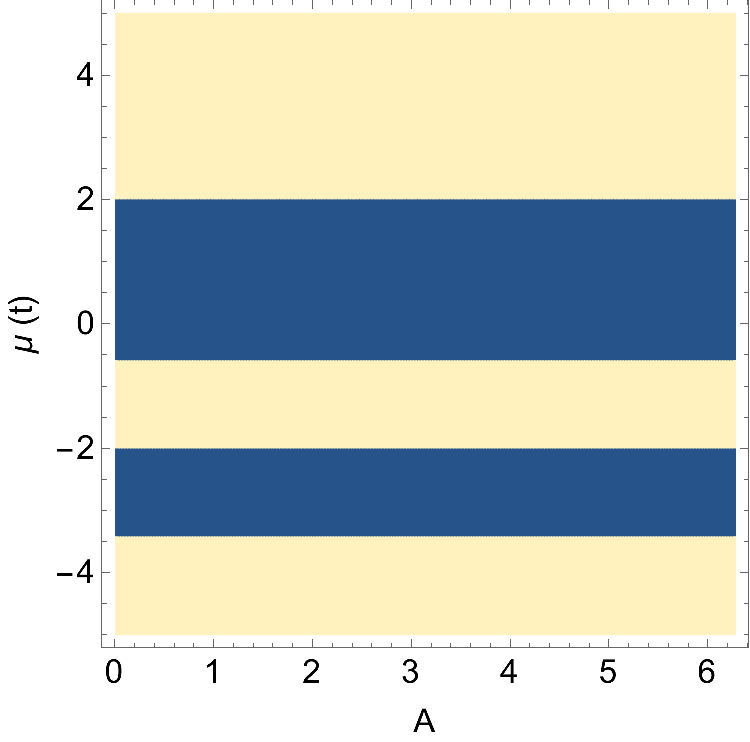
\includegraphics[width=0.3\textwidth]{./figures/majorana-number-y-axis.pdf}%
  }\hfill
  \subfloat[\label{subfig: majorana-number-5pi6ths}]{%
    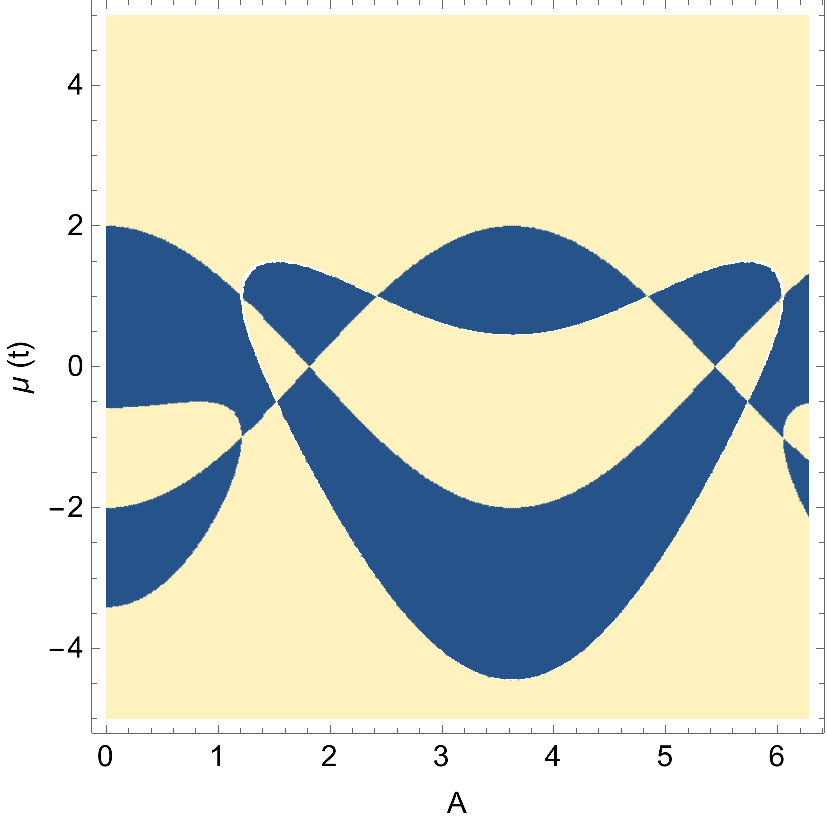
\includegraphics[width=0.3\textwidth]{./figures/majorana-number-5pi6ths.pdf}%
  }\hfill
  \label{fig: majorana-number}
  \caption{Topological phase diagrams for a system with three rows (a) regions III and IV, and (b) regions I and II, from figure \ref{fig: triangular-island-vector-potential-divided}}
\end{figure}

We can now use bulk-edge correspondence to justify the production of Majorana fermions at the interfaces of the triangular islands edges, i.e. corners.
We simulataneoulsy tune regions I and II to be in a trivial phase and regions III and IV to be non-trivial.
To check we look at the numerical eigenenergy spectral flow and eigenstates of a triangular lattice with size $n=100$, and width $w=3$, and $A = [0,2\pi]$.
Figure \ref{fig: spectral-flows} shows strong agreement of MZM's appearing in the same vector potential range as seen in figure \ref{subfig: majorana-number-5pi6ths}'s topological phase diagram.
As expected we find MZM's at the bottom corners of the triangle where the differing topologies meet, as seen in figure \ref{fig: mzm-wavefunctions}.

\begin{figure}[]
  \subfloat[\label{subfig: spectral-flow-mu-0.0}]{%
    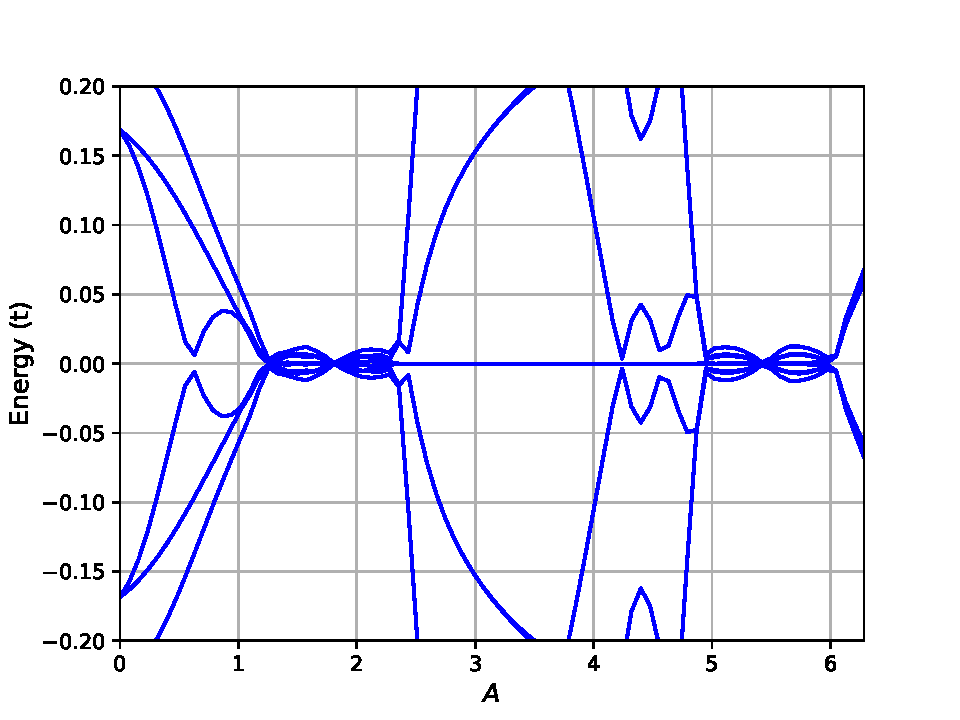
\includegraphics[width=0.3\textwidth]{./figures/spectral-flow-n-100-w-3-mu-0_0.pdf}%
  }\hfill
  \subfloat[\label{subfig: spectral-flow-mu-0.2}]{%
    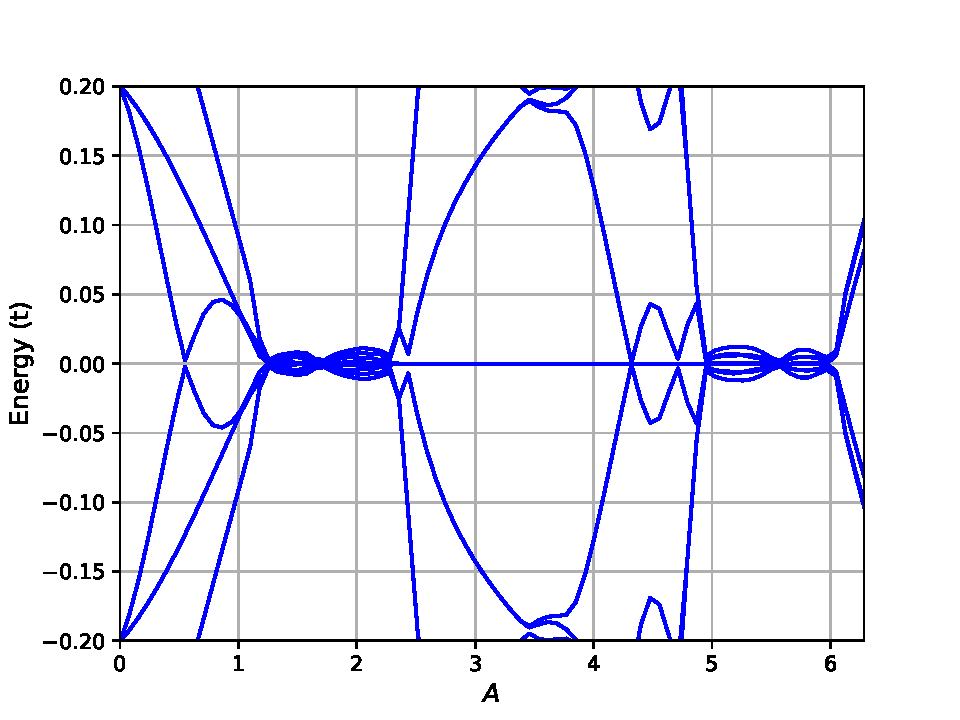
\includegraphics[width=0.3\textwidth]{./figures/spectral-flow-n-100-w-3-mu-0_2.pdf}%
  }\hfill
  \subfloat[\label{subfig: spectral-flow-mu-1.6}]{%
    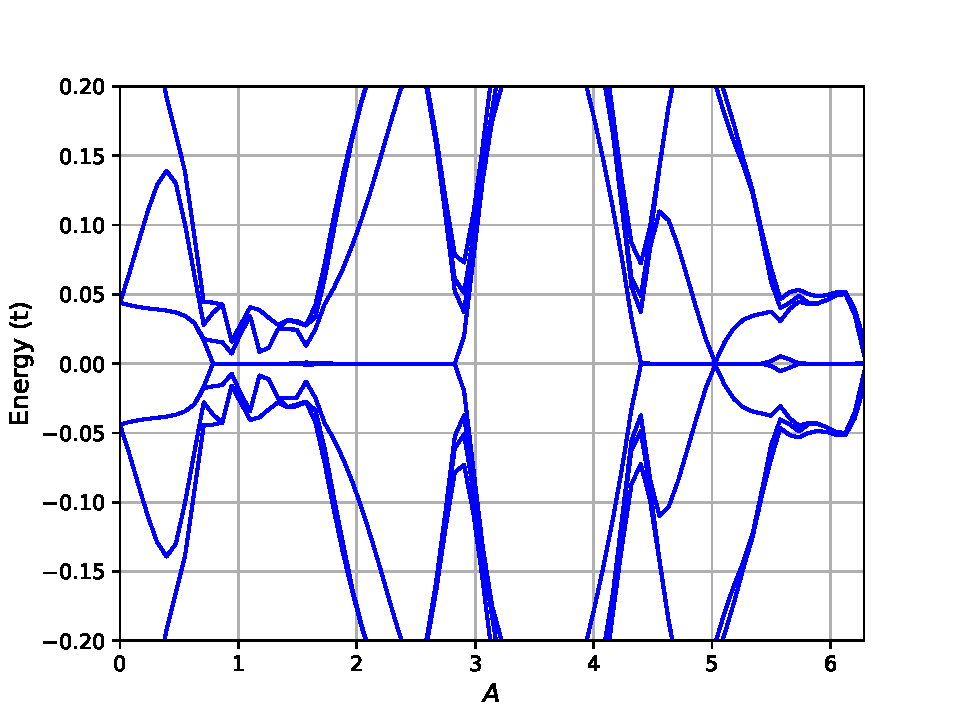
\includegraphics[width=0.3\textwidth]{./figures/spectral-flow-n-100-w-3-mu-1_6.pdf}%
  }\hfill
  \subfloat[\label{subfig: spectral-flow-mu-n1.6}]{%
    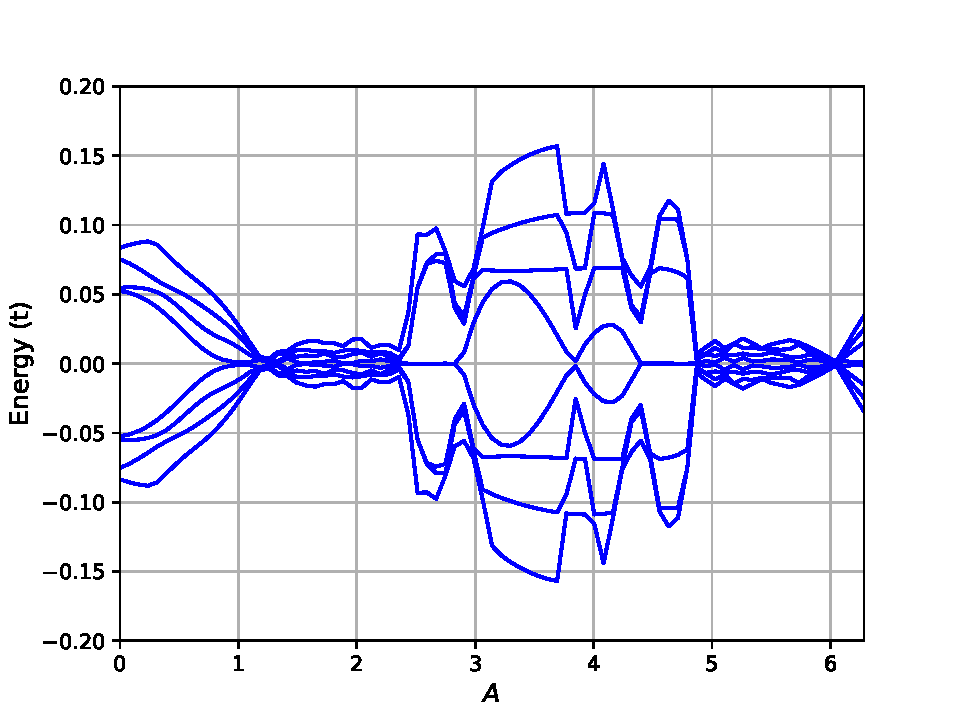
\includegraphics[width=0.3\textwidth]{./figures/spectral-flow-n-100-w-3-mu-n1_6.pdf}%
  }\hfill
  \label{fig: spectral-flows}
  \caption{Eigenenergy spectral flow for a system with $n_r=100$ and $w_{edge}=3$, with (a) $\mu=0$, (b) $\mu=0.2t$, (c) $\mu=1.6t$, and (d) $\mu=-1.6t$.}
\end{figure}

\begin{figure}[]
  \subfloat[\label{subfig: mzm-mu-0.0}]{%
    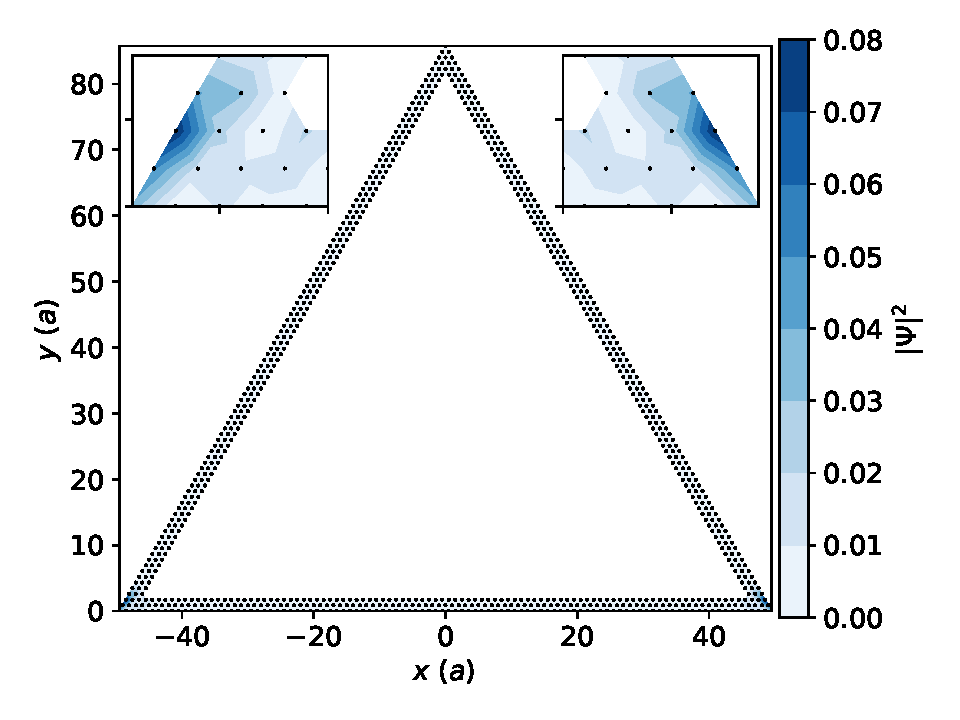
\includegraphics[width=0.3\textwidth]{./figures/En00-B-2_8274-n-100-w-3-mu-0_0.pdf}%
  }\hfill
  \subfloat[\label{subfig: mzm-mu-0.2}]{%
    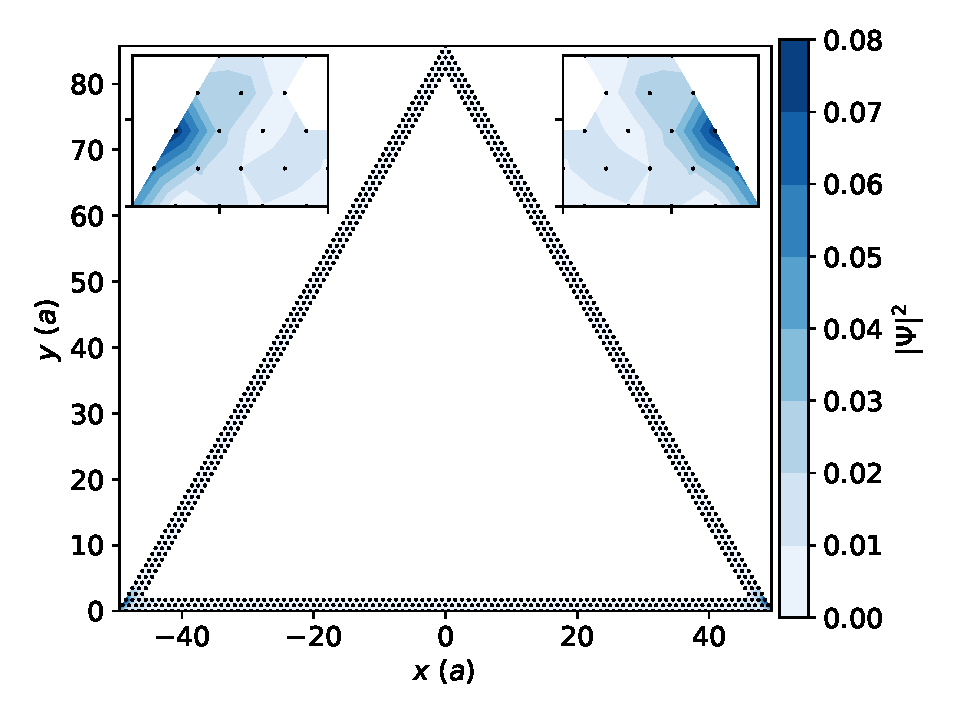
\includegraphics[width=0.3\textwidth]{./figures/En00-B-2_5918-n-100-w-3-mu-0_2.pdf}%
  }\hfill
  \subfloat[\label{subfig: mzm-mu-1.6}]{%
    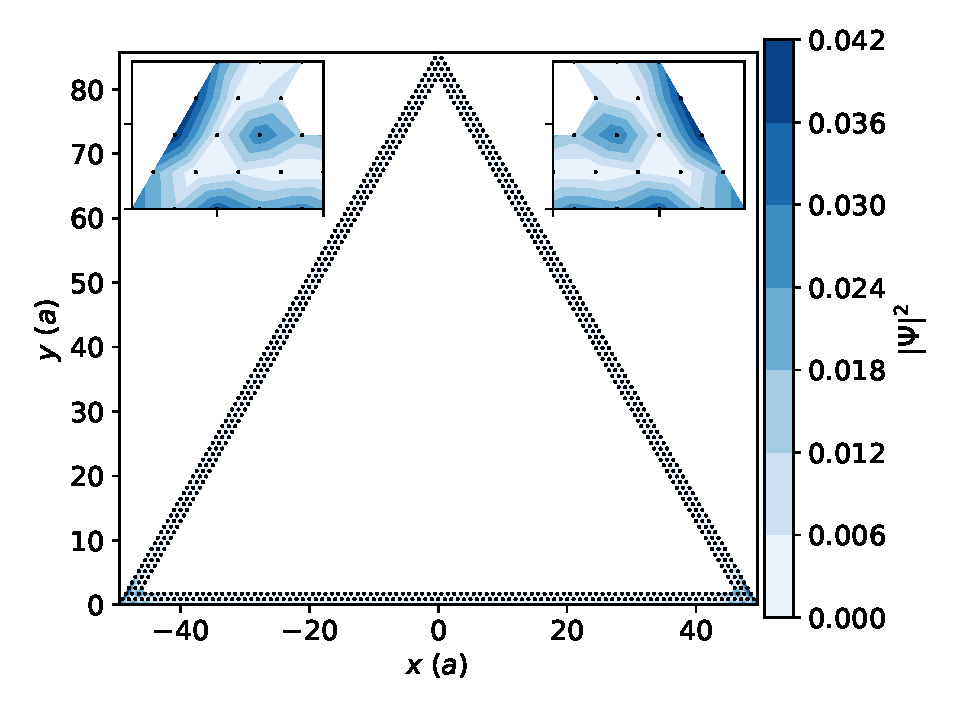
\includegraphics[width=0.3\textwidth]{./figures/En00-B-2_6704-n-100-w-3-mu-1_6.pdf}%
  }\hfill
  \subfloat[\label{subfig: mzm-mu-n1.6}]{%
    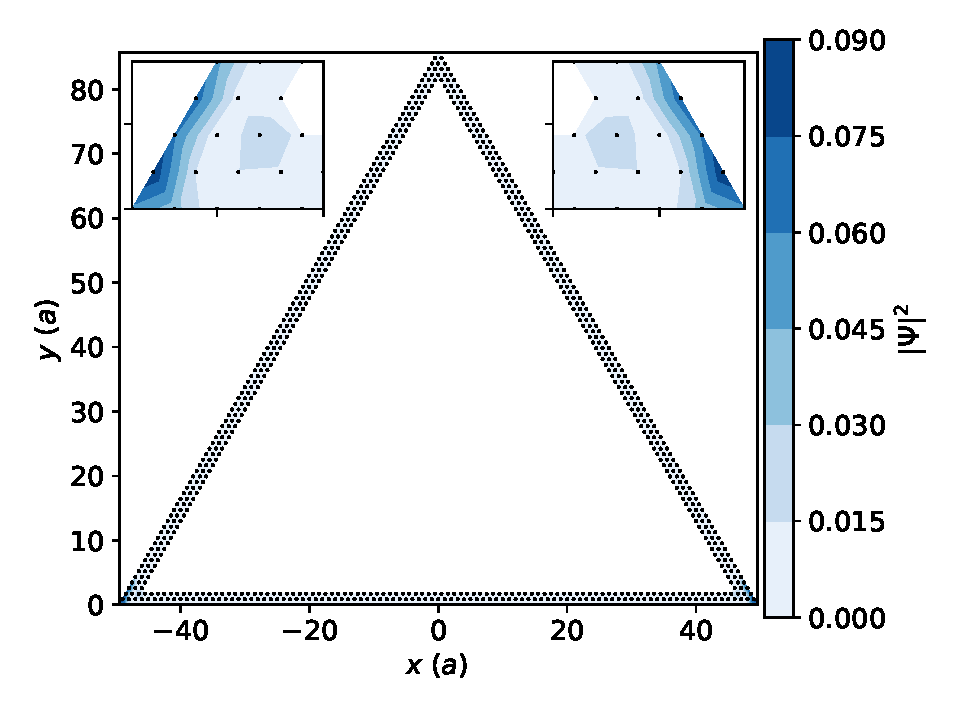
\includegraphics[width=0.3\textwidth]{./figures/En00-B-2_4347-n-100-w-3-mu-n1_6.pdf}%
  }\hfill
  \label{fig: mzm-wavefunctions}
  \caption{MZMs for a system with $n_r=100$ and $w_{edge}=3$, with (a) $\mu=0.2t$, $A = 2.8274$, (b) $\mu=0.2t$, $A = 2.5918$, (c) $\mu=1.6t$, $A = 2.6704$, and (d) $\mu=-1.6t$, $A = 2.4347$.}
\end{figure}

\section{Triangular islands}

\subsection{\Red{3-site problem and kitaev limit for tri.chain, solid triangle}}
We next show we can get exact MZMs in a simple 3-site triangular lattice.
Recall equation \ref{eq: Peierls Hamiltonian}, it is difficult to come to any conclusion while in the complex fermion basis, but if we write our Hamiltonian in Majorana fermion basis we can get a clearer picture.
\Red{Maybe a see supplementary material XX for derivation here.}
The Hamiltonian now takes the form
\begin{align}
  \ham = -\dfrac{i\mu}{4} \sum_j (& a_j b_j - b_j a_j) \nonumber \\
  -\dfrac{i}{4} \sum_{\langle j,l \rangle} [&(t\sin\phi_{l.j}-\de\sin\theta_{l,j}) a_l a_j \nonumber \\
  +&(t\sin\phi_{l,j}+\de\sin\theta_{l,j}) b_l b_j \nonumber \\
  +&(t\cos\phi_{l,j}+\de\cos\theta_{l,j}) a_l b_j \nonumber \\
  -&(t\cos\phi_{l,j}-\de\cos\theta_{l,j}) b_l a_j].
\end{align}
To clear things up, $\phi_{l,j} = -\phi_{j,l}$ since the direction of integration is reversed and the angle $\theta_{l,j} = \theta_{j,l} + \pi$, this ensures we have a Hermitian Hamiltonian.

Let us consider a 3-point triangle lattice, where each lattice point is a complex fermion housing two Majorana fermions.
The bottom left point is $a_1, b_1$, bottom right is $a_2, b_2$, and the top point is $a_3, b_3$.
Similar to Kitaev we will make the same assumptions $t=\de$ and $\mu=0$.
We are left with several combinations of trig terms.
We need some of these combination to go to zero.
Notice how each individual row looks like a Kitaev chain, we need to look at how the rows interact with each other.
Since our goal is to have two Majorana zero modes at the bottom corners, lets aim to have $a_1$ and $b_2$ be such modes.
Anytime $a_1$ or $b_2$ appear in our equation we need its trig terms to cancel, eliminating those particles coupling to the rest of the system.
Let us look at the energy going from site 1 to site 3, $\theta = \pi/3$, we notice the first and last term should be
\begin{align}
  (\sin\phi_{31} - \sin\pi/3) a_3 a_1 = 0, \\
  (\cos\phi_{31} - \cos\pi/3) b_3 a_1 = 0.
\end{align}
This is true if $\phi_{31} = \pi/3$.
Now let's consider the energy from site 3 to site 2.
The phase angle $\theta = -\pi/3$ and the two simplified equations involving $b_2$ are
\begin{align}
  (\sin\phi_{23} - \sin(\pi/3)) b_2 b_3 = 0, \nonumber \\
  (\cos\phi_{23} - \cos(\pi/3)) b_2 a_3 = 0. \nonumber
\end{align}
Here we see $\phi_{23} = \pi/3$.
A constant step-function vector potential one can get with the desired phase is
\begin{equation}
  \vec{A} = \begin{cases}
      \dfrac{2 \pi}{3\sqrt{3}a} \hat{y} \quad &x > 0 \\
      -\dfrac{2 \pi}{3\sqrt{3}a} \hat{y} \quad &x < 0. \\
            \end{cases}
\end{equation}
We find this is still true if we extrapulate from a 3-point triangle to a triangular island because we only need to consider how the coupling of the corner Majorana fermions with its neighboring sites.

\section{Conclusions and Discussion}

\Red{PLACEHOLDER}


\begin{acknowledgements}
  Supported by XYZ Grant No. XXXXXX etc.
\end{acknowledgements}


\bibliography{triag_ref}


\end{document}
